% FH Technikum Wien
% !TEX encoding = UTF-8 Unicode
%

\documentclass[MSC,Master,english]{twbook}%\documentclass[Bachelor,BMR,ngerman]{twbook}
\usepackage[utf8]{inputenc}
\usepackage[T1]{fontenc}
% BERND: Additional Pkg
\usepackage{tcolorbox}
\usepackage{xcolor}
\usepackage{hyperref}
\usepackage{listings}
\usepackage{graphicx}

\lstset{
    captionpos=b,
    numberbychapter=false,
    caption=\lstname,
    frame=single,
    numbers=left,
    stepnumber=1,
    numbersep=2pt,
    xleftmargin=15pt,
    framexleftmargin=15pt, 
    %umberstyle=\tiny,
    tabsize=3,
    columns=fixed,
    basicstyle={\fontfamily{pcr}\selectfont\footnotesize},
    keywordstyle=\bfseries,
    commentstyle={\color[gray]{0.33}\itshape},
    stringstyle=\color[gray]{0.25},
    breaklines,
    breakatwhitespace
}
\lstloadlanguages{bash}

% Define Code-Color
\definecolor{codegreen}{rgb}{0,0.6,0}
\definecolor{codegray}{rgb}{0.5,0.5,0.5}
\definecolor{codepurple}{rgb}{0.58,0,0.82}
\definecolor{backcolour}{rgb}{0.95,0.95,0.92}

% Bitte in der folgenden Zeile den Zitierstandard festlegen
%\newcommand{\FHTWCitationType}{IEEE}
%\ifthenelse{\equal{\FHTWCitationType}{HARVARD}}{\usepackage{harvard}}{\usepackage{bibgem}}
%BERND: TBH that package is 20 years old, get some more up2date packages for cite
\usepackage[utf8]{inputenc}
\usepackage[english]{babel}
\usepackage{csquotes}
%\usepackage[backend=biber,style=ieee,bibstyle=ieee]{biblatex}
%\usepackage[backend=bibtex,style=numeric,bibstyle=ieee]{biblatex}
%ARCH Linux fix
\usepackage[backend=biber,style=numeric,sortcites,natbib=true,sorting=none]{biblatex}
\addbibresource{Literatur.bib}

%Formatieren des Quellcodeverzeichnisses
\makeatletter
% Setzen der Bezeichnungen für das Quellcodeverzeichnis/Abkürzungsverzeichnis
%in Abhängigkeit von der eingestellten Sprache
\providecommand\listacroname{}
\@ifclasswith{twbook}{english}
{%
    \renewcommand\lstlistingname{Code}
    \renewcommand\lstlistlistingname{List of Code}
    \renewcommand\listacroname{List of Abbreviations}
}{%
    \renewcommand\lstlistingname{Quellcode}
    \renewcommand\lstlistlistingname{Quellcodeverzeichnis}
    \renewcommand\listacroname{Abkürzungsverzeichnis}
}
%Wenn die Option listof=entryprefix gewählt wurde, Definition des Entyprefixes für das
%Quellcodeverzeichnis. Definition des Macros listoflolentryname analog zu listoflofentryname und
%listoflotentryname der KOMA-Klasse
\@ifclasswith{scrbook}{listof=entryprefix}
{% 
    \newcommand\listoflolentryname\lstlistingname
}{%
}
\makeatother
\newcommand{\listofcode}{\phantomsection\lstlistoflistings}


%
% Einträge für Deckblatt, Kurzfassung, etc.
%
\title{Kubernetes on the Edge}
\author{Bernd KLAUS, BA}
\studentnumber{2010303012}
\supervisor{Dipl.-Ing. Hubert Kraut}
\secondsupervisor{Dipl.-Ing. Andreas Happe}
\place{Wien}

\kurzfassung{
Kubernetes wird als Schweizer Armemesser der Container-Orchestrierung bezeichnet. Auch im Bereich edge-computing bietet der Dienst eine Vielzahl an unterschiedlichen Werkzeugen und Tools an, welche Teils unterschiedliche Strategien und Ansätze verfolgen. Die Auswahl reicht von einem zentralen Kubernetes-Cluster der verteilte Geräte, sogenannte „Leafs“, steuert bis hin zu vielen einzelnen und verteilten kleinen Clustern an der Edge, welche zentral gesteuert werden. Entscheidend ist es den richtigen Anwendungsfall zu erheben, um sich für die optimale Lösung entscheiden zu können. Ebenfalls spielen sicherheitstechnische Aspekte bei derart komplexen Umgebungen eine wichtige Rolle. Die vorliegende Arbeit gibt Einblicke und Entscheidungsgrundlagen sowie Empfehlungen hinsichtlich der IT-Security. Belegt werden die Angaben durch Implementierung eines Proof-of-Concepts
}
\schlagworte{Kubernetes, edge-computing, distributed System, Proof-of-Concept}


\outline{
Kubernetes is the de facto swiss-army-knife for orchestrating container-platforms. In addition, Kubernetes can also be used for deploying devices as well as applications on top of it on the edge of the network. However, there are different methods for archiving comparable results. On the one hand a possible solution is to build a central instance managing small distributed and independent clusters, on the other hand a centralized cluster with just leafs on the edge may be a better fit. This results in the challenge to find the best solution for the desired environment respectively use-case. The following thesis is making use of "Design Science Research" to give introductions on how to choose the proper architecture for the aimed environment.
}
\keywords{Kubernetes, edge-computing, distributed System, Proof-of-Concept}

%
% Start the Thesis
%

\begin{document}
\maketitle
\chapter{Introdutcion}
\label{chap:introduction}
Because of \ac{IoT} Devices becoming more and more common, the number of devices capable of communicating with the \ac{WWW} increases rapidly. Consequently, also the overall traffic generated as well the amount of data which must be processed increases accordingly. Regarding this development edge-computing is the rising start trying to solve that issues. Thereby data is not processed centrally like in traditional datacenters, but it is tried to handle those data close to the user within several distributed systems. Because of this methodology only really necessary data is transmitted to a central instance for further treatment and those the processing-power as well as the bandwidth necessary for processing required data is reduced significant. \par It is expected that the number of IoT devices will continue to grow fast \cite{SotE21} over the coming years. Concomitant edge-computing also will become more important in the future and become an important role in modern \ac{IT} architectures. \par To be able to control distributed systems effectively \ac{K8s} is providing a lot of useful tools and functions. Fundamentally there are two different approaches regrading the architecture of how to build an edge-computing environment making use of \ac{K8s}:

\begin{itemize}
    \label{item:architecture}
    \item \textbf{Default}: A centralized \ac{K8s} Cluster controlling many leaf-devices (workers) on the Edge.
    \item \textbf{Distributed}: Small and distributed \ac{K8s} Clusters running independent on the Edge controlled by a centralized Master-Instance.
\end{itemize}

Another upcoming approach of solving that issue is making use of the service mesh \cite{servicemesh}. This ultimately uses or builds on both of the aforementioned technologies. However, since this thesis concentrates on the two main architectures and their differentiation, the service mesh is not the main focus and just mentioned for the sake of completeness.

\section{Problem area}
Problems arise when trying to find the proper architecture for a specific use-case. There is no clear winner when comparing the above-mentioned different variants. Each of them  has their own pros and cons and may decide whether a project is successful or not. It is therefore all the more important to choose the proper architecture right before starting, changing the strategy in retrospect would take a lot of time and effort. However, there is no clear guidance on how to find the proper target environment, at least none which apply in general. Occasionally one finds recommendations for a very specific use case, however the chance is slim low this findings fit your goals respectively enlighten the decisions. This leads us to the following research question.

\section{Research question}
\label{sec:rq}
This paper is going to answer the subsequent research questions:
\begin{enumerate}
    \item What are the main differences of the in chapter \hyperref[item:architecture]{one} mentioned architectures regarding functionality, scalability, costs and security?
    \item Which decision criteria must be defined respectively examined to create a catalog capable
    of choosing the proper architecture easier for \ac{IT} managers as well as administrators?
    \item Is there a trend in which technology is most likely to be used?
\end{enumerate}

\section{Goal}
\label{sec:goal}
The main goal of this thesis is to highlight the pros and cons for each of the \hyperref[item:architecture]{architectures} defined in the \hyperref[chap:introduction]{Introduction}. The focus will be mainly on the geo-distribution aspect. Although \ac{IoT} is playing a major role in pushing the development forward, however it is not considered further in the present work. To find the proper architecture, or at least recommendations what could fit best for different desired use-cases, a catalog will be defined. An important part will become the decision tree helping people making comprehensible decisions based on scientific research. The main characteristics which are taken into account are scalability, state-of-the-art, handling, costs as well as security.

\section{Methodology}
\label{sec:methodology}
In the first part of the present work existing literature will be inspected. Related and relevant work will be examined accordingly and linked in the document. Also results will be incorporated to get out the most of it. In the second part a catalog with main criteria necessary for decision-making is defined. Part of this catalog will also be a decision-tree, mentioned in the previous chapter, to easily find the proper architecture. The last chapter (\hyperref[sec:dsranalysis]{Analysis}) deals with testing the defined criteria against real world examples making use of the \ac{DSR} methodology. The last chapter is given the most attention, it is the area where new techniques or architectural decisions are finally verified and the proof is given whether the catalogue works as expected or not. In the latter case, the catalog will be revised to reflect the findings of the last step and re-examined again using \ac{DSR}.


\chapter{State of the Art}
\label{chap:current}
The first chapter (\hyperref[chap:introduction]{Introduction}) gives a brief introduction to the main technologies used respectively examined in the later part of the document. If anyone is already familiar with the subject may you jump over to the \hyperref[sec:architecture]{Architecture} chapter.
\section{Technology}
\label{sec:technology}
\subsection{Kubernetes}
To promote modern development and be able to implement continuous deployment pipelines cumbersome monolithic applications are divided into many smaller units. Each of these units provides only one function. In order to establish the overall functionality, these units are communicating with each other and thus provide services or make use of other ones. This new method of delivering applications brings many advantages in terms of development but also introduce some new challenges and complexities regarding operation. To simplify the tasks around the management of this architecture, \ac{K8s} has established itself as the de facto standard \cite{k8ssurv}. \ac{K8s} was initially developed by Google and later donated to the opensource community. Over the course of time, a broad community has developed around \ac{K8s} and a number of additional tools and extensions have emerged as a result. The most promising solutions regrading geo-distribution respectively edge-computing are highlighted in the subsequent section \hyperref[sec:architecture]{Architecture}. In order to be able to interpret the results of the use-cases, as well as building the necessary basic understanding, the following functionalities and components of \ac{K8s} are of relevance.  

\begin{figure}[ht]
    \centering
    \tcbox[sharp corners, boxsep=4mm, boxrule=0.2mm, colframe=gray!20!gray, colback=white]{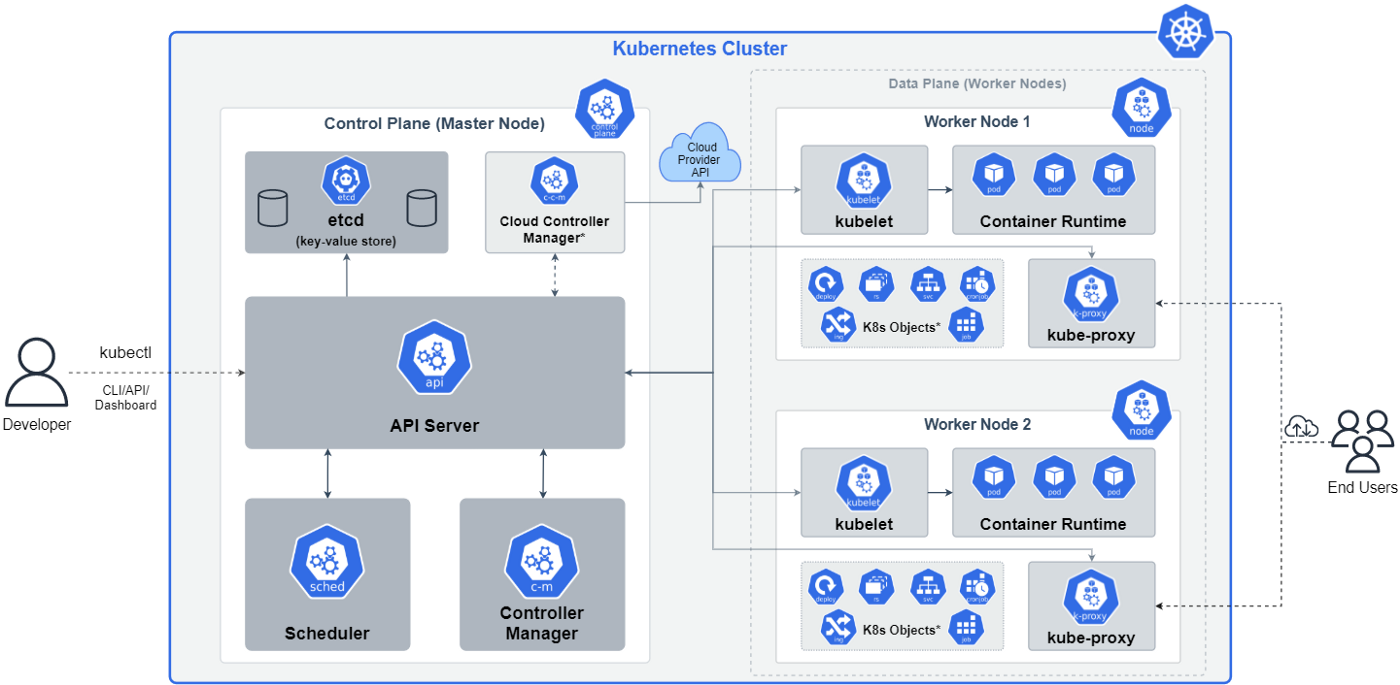
\includegraphics[width=0.75\textwidth]{PICs/k8s-architecture.png}}
    \caption{\ac{K8s} architeture overview \cite{pic-k8s-overview}}
    \label{fig:k8s-architecture}
\end{figure}

\paragraph{Master Nodes} run the so-called \textit{Control Plane} which is responsible for controlling the cluster itself and all the ressources within. The Control Plane consist of the following components \cite{k8scomp}.
\begin{itemize}
    \item \textit{kube-apiserver} acts as frontend web-interface responsible for controlling the \ac{K8s} cluster as well as the objects inside the cluster. Tools like kubectl abstract the \textit{OpenAPI v2} endpoint and provide access in form of a simply understandable and usable \ac{CLI}. 
    \item \textit{etcd} represents a high-available and consistent key value store responsible for storing the actual state as well as the desired configuration of the cluster.
    \item \textit{kube-scheduler} is responsible for scheduling pods on the available worker nodes. Decision variables such as available ressources, affinity-rules and constraints are taken into account. However, the default \textit{kube-scheduler} ist not aware of any latency between the worker nodes nor the pods communicating with each other. As discovered in the following chapters, this appears to be an important variable for edge-deployments. However, some available white-papers already try to address those issues and show possible solutions by adopting a custom scheduler taking care of those values. More details on this can be found in the chapter \hyperref[chap:related]{Related Work}.
    \item \textit{kube-controller-manager} consists of a single compiled binary controling the status of nodes, jobs, service-accounts and endpoints as well as creating or removing them.
    \item \textit{cloud-controller-manager} represents the interface to the underlying cloud-platform. This allows kubernetes to create and/or configure load-balancers, routes and persistent-volumes on the underlying cloud-infrastructure. In a local environment e.g. minikube \cite{minikube} provide the \textit{cloud-controller-manager} becomes an optional component and is not required. The same may apply to edge-locations as those areas are outside the cloud most of the time.
\end{itemize}

\paragraph{Worker Nodes} manage the workload, i.e. run the actual application(s). These nodes are composed of the following, see list below, parts \cite{k8scomp}. It should be mentioned, that also the described \textit{Master Nodes} are executing those components because some core-componentes are containerized (pods) itself. 
\begin{itemize}
    \item \textit{kubelet} is an agent which assures that the container is executed properly inside their associated pods according to its specifications defined via \textit{PodSpec}. Also \textit{kubelet} is responsible for monitoring the healthy state of the containers.
    \item \textit{kube-proxy} uses the packet filters of the operating system underneath to forward traffic to the desired destination. The resulting access points, also called \textit{Services} in \ac{K8s}-jargon, can be made available either internally or externally.
    \item \textit{container runtime} is the part that finally executes the containers. The default runtime at time of writing is \textit{containerd}, however any runtime is supported that complies with the CRI specification \cite{cri-runtime}.
\end{itemize}

\paragraph{Kubernetes Objects} are persistent properties inside the \ac{K8s} ecosystem representing the state of a cluster. The most important feature of those objects is to describe the target environment in a declarative way. For this purpose, most of the time, YAML files are used. Kubernetes now ensures that the desired state of the environment is actually achieved and continuously monitors the required objects to meet those defined requirements. This mechanism is also ideal for distributed systems, such as edge computing, as availability can be monitored at any time and a an action can be taken if necessary. Subsequent the main objects are cited starting with the smallest unit \cite{k8sconc}.
\begin{itemize}
    \item \textit{Containers} decouple the actual application and its dependencies from the underlying infrastructure. The main properties of those containers are there immutability and repeatability. This means that the container can be rebuilt at anytime resulting in an identical clone. Likewise, the code of a running container cannot be modified subsequently.
    \item \textit{Pods} include at least one or more \textit{Containers}. In the most scenarios a single pod consists of a single container, in some cases a so-called sidecar container is used increasing the number of containers inside a pod. Containers which are in the same \textit{Pod} share the same local Socks as well as volumes mounted.
    \item \textit{Deployments}, \textit{Statefulsets} and \textit{Daemonsets} are responsible for ensuring the actual workload is provided, to achieve this they control and scale the assigned \textit{Pods}. When creating an application for \ac{K8s}, it is most likely to create one of those objects. The \textit{Pods} and \textit{Containers} are merely an end product that is derived these objects.
    \item \textit{Services} provide an abstract way to make a set of \textit{Pods} available on the network via a single endpoint. Additional deployed pods will automatically be added to the responsible \textit{Services}. Thereby \ac{K8s} is an excellent choice when it comes to scaling applications without any manual intervention. This also applies for deploying applications to the edge of the network, as illuminated in the course of this thesis. Closely related to the \textit{Services} is the \textit{Ingress} resource, which is taking care of making the aforementioned objects available outside the cluster. An optional reverse-proxy (\textit{Ingress-Controller}) must be installed in order to make use of the latter. \newline
    A new feature, which is of relevance regarding edge-computing, currently in beta phase, is the so-called \textit{Topology Aware Hint}. Basically its meta-data added to the endpoints defined previously suggesting the connection client on how to reach the destination efficiently (e.g. zones aware of different locations can be defined)
    \item \textit{ConfigMaps} and \textit{Secrets} are pieces of information which can be mounted into to \textit{Container} to adjust the configuration inside at runtime. Even whole files can be replaced using on of them. \textit{Secrets} are only different in the sense that they decode the content, however technically they are the same.
    \item \textit{Volumes} provide persistent storage which extends beyond the life cycle of the pods. Volumes can be mounted at any defined position inside the pods. The disadvantage is that the data written to those \textit{Volumes} resides out of the \ac{K8s} ecosystem and therefore the operator must take care of data security and replication. This becomes even more complicated in an edge-computing environment where nodes have higher latency between them.
\end{itemize}

\subsection{Edge-Computing}
Edge-computing is the model that extends cloud services to the edge of the
network. The computing resources on the edge act as a layer between the user, who provides or wants to process data, and the centralized datacenter (e.g. the cloud). Because data can be processed earlier respective closer to the user, latency and amount of data transferred can be reduced \cite{intro-edge}. Also, the required computing-ressources in the datacenter can be minimized because data can be processed at the edge. A major driver of the subsequent s technology is \ac{IoT}. The amount of devices and resulting data volume, which must be processed, is increasing exponentially \cite{SotE21}. Another technology which depends on it are low-latency applications like e.g. video-streaming. 

\paragraph{Hierarchy} descripes the layers of the architecture. The following list enumerates the most important layers from top to bottom \cite{intro-edge}.
\begin{enumerate}
    \item \textit{Cloud} - centralized datacenter
    \item \textit{Fog} - distributed "smaller" datacenters
    \item \textit{Edge} - the closest unit to the end-user
    \item \textit{\ac{IoT}} - device at the edge put into use
\end{enumerate}


The main focus of this work is to efficiently combine the two layers \textit{Cloud} and \textit{Edge} and orchestrate between them using \ac{K8s}. The layer \textit{Fog} is skipped because it is often seen to be "the same" as the \textit{Edge}. Also, current \ac{K8s} based solutions do not make use of it. 

\paragraph{Geo-Distribution} characterises the aspect of the geographical propagation of the edge ressources. The goal is to provide computing power over wide areas, each close to the users. By establishing many of these locations in different regions, network latency can be significantly reduced from the user's perspective. However, the latency between the edge-nodes and the centralized cloud still remain.


\section{Architecture}
\label{sec:architecture}
\subsection{Default}
In order to be able to manage resources at the edge, a traditional architecture can be used. This is subdivided into a centralized \textit{Control Plane} hosted in the cloud and distributed worker nodes near the edge. The same \ac{K8s} architeture is commonly used when deploying to a single location aswell inside the cloud. The following graphic illustrates the architecture.

\begin{figure}[ht]
    \centering
    \tcbox[sharp corners, boxsep=4mm, boxrule=0.2mm, colframe=gray!20!gray, colback=white]{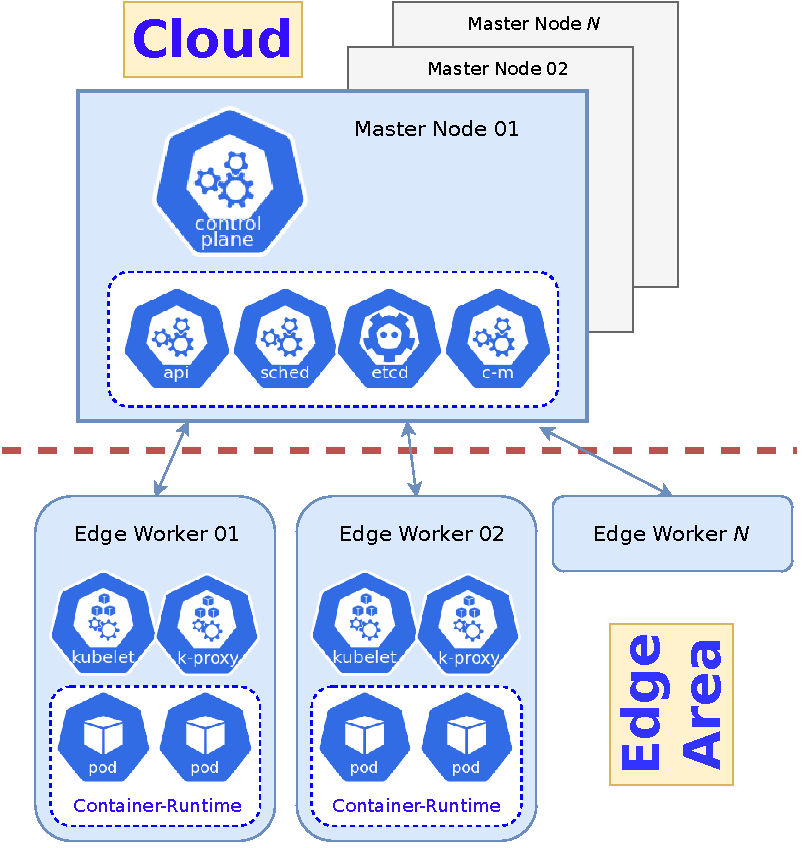
\includegraphics[width=0.75\textwidth]{PICs/drawio/defaul-k8s.drawio.pdf}}
    \caption{Default \ac{K8s} architeture}
    \label{fig:k8s-default}
\end{figure}

Although the conventional components can also communicate with each other over long distances, there are still some challenges that need to be taken into account. An important role in this context is played by the \ac{CNI}. This part of \ac{K8s}, which can be selected in the form of a plugin, is responsible for the cluster-internal network traffic. Some of these plugin providers offer advanced features that facilitate geographical distribution. Some of the most used \ac{CNI} providers are \cite{k8s-cni}:

\begin{itemize}
    \item Calico
    \item Canal
    \item Cilium
    \item Flannel
    \item Weave
\end{itemize}

In contrast to the plugins mentioned above, KubeEdge was developed explicitly for deployments on the edge \cite{kubedge}. The main advantages are:

\begin{itemize}
    \item KubeBus - a custom network plugin working in private \ac{IP} address ranges behind \ac{NAT}. Thereby no dedicated public ip is necessary for edge locations making the architecture more flexible.
    \item SyncService - Another important part of KubeEdge is the metadata sync service running on each worker node. This extension cyclically synchronises the data of the master. Thus, the quantity of data to be called up can be minimized and workload can continue to run in offline scenarios.
    \item Lightweigt Agent - TODO
\end{itemize}

challanges
Storage is an issue (latency: asynch)
DNS issue
Services Issues (not awar of location)



Target length: 2-4 S (incl. picture)
\subsection{Distributed K8s}
Cluster running indepented - KubeFed
Completely different approach, no network necessary beween at all.
Target length: 2-4 S (incl. picture)
\textcolor{red}{TODO: Picture Distributed}

\section{General Challenges} 
Challenges that appear when creating respectively operating such infrastructures are diverse, as can be seen in the following list \cite{intro-edge}.

\begin{itemize}
    \item Variety - a lot of different locations, technologies as well as methods on how to control devices on the edge is challenging for both development and operation. The better these different factors can be abstracted and simplified, the more effectively the infrastructure can be used.
    \item Integration - edge-computing evolves very quickly, thereby things could change quickly. The more important it is to keep the provided interfaces extensible. This way, new devices or application can be put in use swiftly. 
    \item Awareness - the devices and/or end-user do not care about how their traffic is routed, or their data is processed. However, the architecture needs to take care of that to use the topology in the best possible way.
    \item Resources - scaling Resources like \ac{CPU}, \ac{RAM} and disk space at the edge is by far more elaborate than in a datacenter or in the cloud.
    \item \ac{QoS} - The service provided at the edge should be reliable and provide a good user experience. Availability and performance play a central role in this context. As the availability can not be guaranteed to some extent, an appropriate failover mechanism should be in place.
    \item Security - physical access control as well as isolating applications from each other is a difficult task. Also, the data traffic must be separated accordingly. In general, \ac{IT} security is a hot topic, and especially at the edge, it requires appropriate consideration for hardening the environment.
    \item Monitoring - another important factor is how to capture metrics and events (logs) from the edge. They need to be indexed on a centralized instance in order to get a general overview on what's happening. Because of the dynamic and rapid changes some kind of automatic discovery should be used for that purpose.
    \item Environment - Some locations may have to deal with difficult conditions regarding their surroundings. Increased dust exposure, poor internet connections or recurring power outages can be some of these factors. The system must be able to cushion or parry such failures accordingly.
\end{itemize}
The above-mentioned challenges provide a good starting point for defining the necessary tests to find the matching target architecture. Details about this test can be found in the chapter \textit{\hyperref[sec:dsrmethode]{Methodlogy}}.



\chapter{Design Science Research}
\label{chap:dsr}

\section{Methodology}
\label{sec:dsrmethode}
\subsection{Performed Tests}
Target length: 2 S

\section{Environment}
\label{sec:env}
describe the test-environemtn
Target length: 0,5-1 S

\section{Architecture}
\label{sec:dsrarchitecture}
\subsection{Default}
Target length: 3-4 S
\subsection{distributed K8s}
Target length: 3-4 S


\section{Use-Cases}
\subsection{Web-Application}
Target length: 1
\subsection{Enterprise VPN}
Target length: 1
\subsection{Distributed Database}
Target length: 1

\section{Analysis}
\label{sec:dsranalysis}
Target length: 4 S
\subsection{Relevant Magnitudes}
\subsection{Performed Tests}
\subsection{Outcome}
\subsection{Paraphrase}



\chapter{Catalog}
\label{chap:catalog}

\section{Decision Variables}
\label{sec:variables}
 
Target length: 1-2 S

\section{Decision Tree}
\label{sec:tree}
Target length: 1 S

\section{Exclusions and Special Cases}
\label{sec:exclusions}
Target length: 1 S



\chapter{Related Work}
\label{chap:related}
Target length: 3 S (all subsections)
\section{Kubernetes and the Edge?}
Some introdution to K8s at the Edge, highlighting the main Architectures.
\section{Extend Cloud to Edge with KubeEdge}
Descripes KubeEdge and its advantages
\section{Sharpening Kubernetes for the Edge}
Sharpening Kubernetes for the Edge
Make Kubernetes aware of the latency between the nodes at the Edge.
\section{Ultra-Reliable and Low-Latency Computing in the Edge with Kubernetes}
Similar to the paper before. Latecny awar pod deploymentm, but you also can deploy to regions and an custom re-scheduler is implementated taking care of redeploying when one node fails.
Clustering node-groups based on latency.
\section{Latency-aware Optimization of the Existing Service Mesh in edge-computing Environment}
RoutingAgent (Docker Image) extending Isito Service mesh with dynamic weight based routing.
"With the RoutingAgent running in the system, the weights of the target routing clusters will be dyamically changed based on the detected inter-cluster network latency"
TODO: Service Mesh ggf entfernen.

\chapter{Results}
\label{chap:results}

Target length: 3 S (all together)
\section{Findings}
\label{sec:findings}

\section{Conclusio}
\label{sec:conclusio}

\section{Discussion and further research}
\label{sec:discuss}

\paragraph{Notes}
---to-be-removed---
Sites:
- longest: 50 (may i need even more)
- shortest: 36 (zu wenig)
-------------------

Picture example:
\begin{figure}[ht]
    \centering
    \tcbox[sharp corners, boxsep=4mm, boxrule=0.2mm, colframe=gray!20!gray, colback=white]{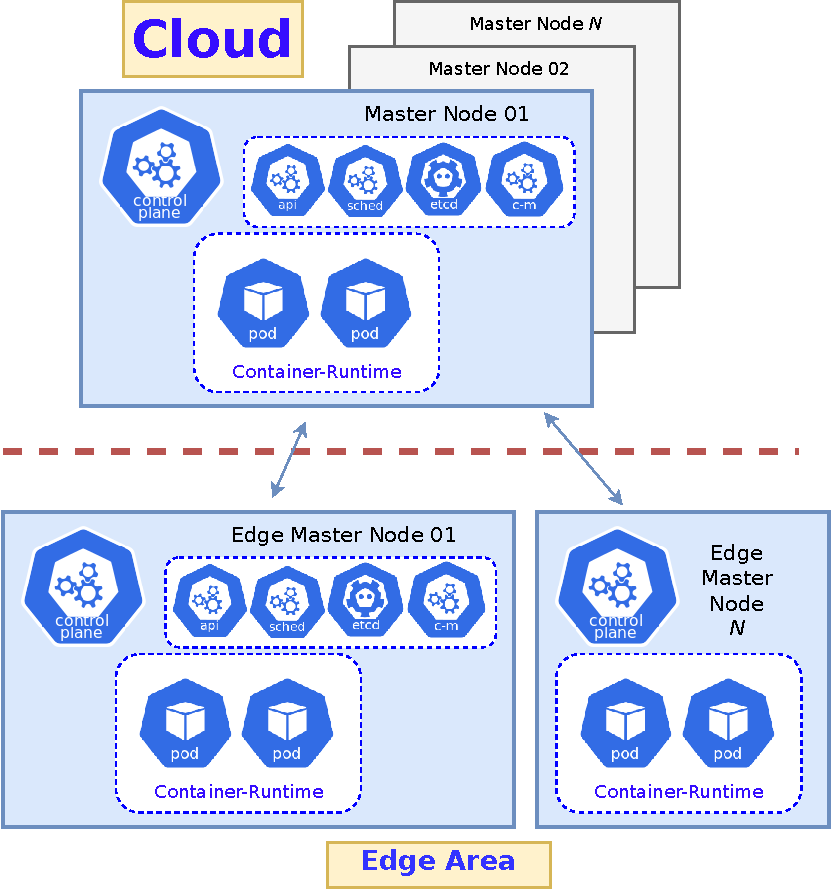
\includegraphics[width=0.75\textwidth]{PICs/drawio/distributed-k8s.drawio.pdf}}
    \caption{Distributed \ac{K8s} architeture}
    \label{fig:distributed-k8s}
\end{figure}

%
% Hier beginnen die Verzeichnisse.
%
\clearpage
%\ifthenelse{\equal{\FHTWCitationType}{HARVARD}}{}{\bibliographystyle{biblatex}}
%\bibliography{Literatur}
\printbibliography 
\clearpage

% Das Abbildungsverzeichnis
\listoffigures
\clearpage

% Das Tabellenverzeichnis
\listoftables
\clearpage

% Das Quellcodeverzeichnis
\listofcode
\clearpage

\phantomsection
\addcontentsline{toc}{chapter}{\listacroname}
\chapter*{\listacroname}
\begin{acronym}[XXXXX]
    \acro{IT}[IT]{information technology}
    \acro{WWW}[WWW]{world wide web}
    \acro{K8s}[K8s]{Kubernetes}
    \acro{IoT}[IoT]{internet-of-things}
    \acro{DSR}[DSR]{Design Science Research}
    \acro{CLI}[CLI]{Command Line Interface}
    \acro{QoS}[QoS]{Quality of Service}
    \acro{CPU}[CPU]{Central Processing Unit}
    \acro{RAM}[RAM]{Random Access Memory}
    \acro{CNI}[CNI]{Container Network Interface}
    \acro{IP}[IP]{Internet Procotcol}
    \acro{NAT}[NAT]{Network Address Translation}
\end{acronym}

%
% Hier beginnt der Anhang.
%
\clearpage
\appendix
\chapter{Appendix}
\clearpage
\chapter{Appendix}
\end{document}